\chapter{DETECTOR}
\label{chap:detector}
The Large Hadron Collider (LHC) is a proton-proton synchrotron located along the French/Swiss border near Geneva, Switzerland which utilizes the same accelerator tunnel that was originally built for LEP.
The collider operates by using superconducting magnets to steer opposing beams of protons around a 27 kilometer circumference. 
The protons are accelerated by means of radio-frequency resonating cavities.
The protons in the LHC have a maximum energy (design) of $7$ TeV in each direction, providing a center of mass collision energy ($\sqrt{s}$) of $14$ TeV.
The analysis presented in this text will focus on the data taken at the Compact Muon Solenoid experiment in 2011, during which time, the center of mass collision energy of the LHC was $7$ TeV.
A common figure of merit for the performance of an accelerator is the luminosity, which can be simply described as the number of particles per unit area per unit time.
The LHC design luminosity is $10^{34}$ \lumiunit, while during the 2011 data taking the peak luminosity reached approximately $5\times 10^{33}$ \lumiunit.
The LHC has four collision points located around its circumference, at these points the proton beams are confined and collided.
There is a detector situated around each of these collision points: The Compact Muon Solenoid (CMS), A Toroidal LHC Apparatus (ATLAS), LHC-B, and A Large Ion Collider Experiment (ALICE).

The analysis presented in this thesis was performed on the CMS detector, thus a brief description of the detector will be given.
The CMS detector is one of two general purpose detectors, the other being the ATLAS detector.
Being a general purpose detector, the CMS detector is designed to observe a wide range of physics processes. 
The CMS detector has a hermetic design such that it is capable of measuring nearly any and all particles that arise from the collisions with little acceptance loss.
A cartesian coordinate system is defined for the CMS detector as follows: the $z$ axis points along the beam pipe, the $y$ axis pointing up with respect to gravity, and the $x$ axis pointing towards the center of the LHC ring.
The CMS detector is designed in the shape of a cylinder, and as such a cylindrical coordinate system is also defined.
The $z$ axis of the cylindrical coordinate system is the same as the $z$ axis of the cartesian coordinate system.
The polar angle ($\theta$) is measured with respect to the $z$ axis with $\theta = 0$ being the positive $z$ axis, and $\theta = \pi$ being the negative $z$ axis.
The azimuthal angle ($\phi$) is measured with respect to the $x$-$y$ plane, $\phi = 0$ is the positive $x$ axis and $\phi = \frac{\pi}{2}$ is the positive $y$ axis.
Rather than the polar angle, it is often more useful to consider the pseudorapidity, $\eta = -ln\left[tan\left(\frac{\theta}{2}\right)\right]$, which for high energy particles approximates the rapidity $y = \onehalf ln\frac{E+p_{T}}{E-p_{T}}$. 
Pseudorapidity is useful in that it is related to the relativistic boost of a particle.
To accomplish the task of observing and measuring the properties of different processes and particles the CMS detector has multiple subsystems dedicated to different tasks.
The inner-most sub system is a tracking device that measures the trajectory of charged particles.
Just outside the tracking system are two calorimeters, first the electric calorimeter (ECAL) which measures the energy of photons and electrons. 
The calorimeter system is completed by the hadronic calorimeter (HCAL) which measures the energy of jets of hadrons and is situated just outside the ECAL.
A superconducting solenoid magnet provides a powerful magnetic field which bends the trajectory of charged particles allowing the measurement of a charged particle's momentum and charge.
The solenoid magnet encloses the tracking system and calorimeter systems.
Finally outside the solenoid is the muon system which measures the trajectory of particles that escape the calorimeters.
Since the calorimeters are designed to completely absorb the energy of all other particles, with limited exceptions the only particles that reach the outer muon system are muons.
A labeled schematic of the CMS detector and its subsystems is given in Figure \ref{fig:cmsdetector}.
\begin{figure}[ht]
\centering
%\begin{center}
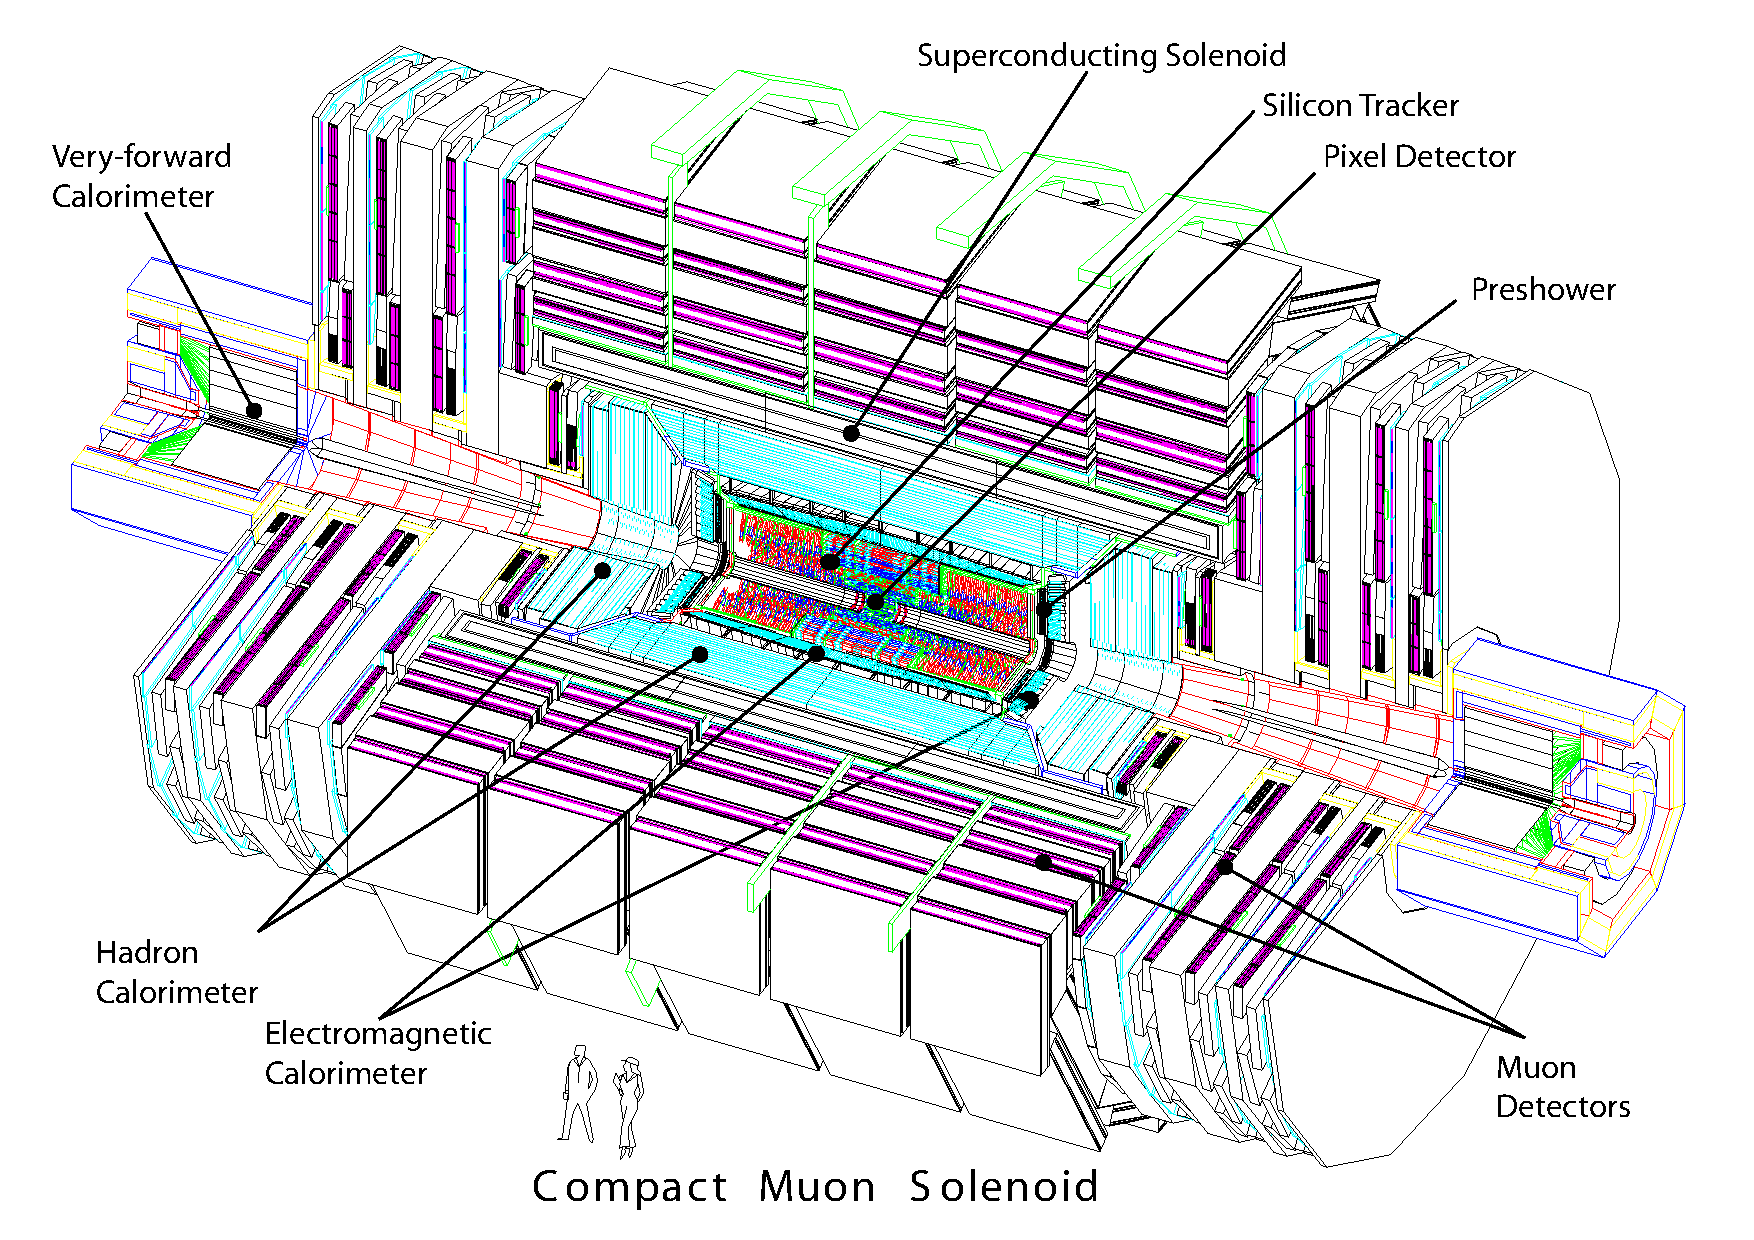
\includegraphics[width=0.9\textwidth]{plots/cmsdetector.pdf}
\caption{Schematic of the CMS detector\cite{CMS_DETECTOR}.}
\label{fig:cmsdetector}
%\end{center}
\end{figure}
\section{The Large Hadron Collider}
\label{sec:lhc}
Protons are delivered to the LHC by means of multiple intermediate accelerators: the Lineac2, the Proton Synchrotron Booster, the Proton Synchrotron (PS), and the Super Protron Synchrotron (SPS).
The PS was the first circular particle accelerator built at CERN in the late 1950s. 
In its current implementation the PS takes protons that originate in the Lineac2 linear accelerator at $50$ MeV that are then accelerated in the Proton Synchrotron Booster to $1.4$ GeV.
The protons are fed from the PS to the SPS which was commissioned in 1976 and has served to accelerate protons, antiprotons, electrons and positrons for various accelerators over its history.
Most notably the SPS accelerator provided the proton-antiproton beams that were used for the UA1 and UA2 experiments that accomplished the discovery of the $W$ and $Z$ bosons.
The SPS later provided the $e^{+}e^{-}$ beams that were used for LEP.
The two proton beams for the LHC are accelerated to their injection energy of $450$ GeV in the SPS at which point the radio-frequency resonating cavities of the LHC accelerate the beams to their collision energies.
A diagram of the CERN accelerator complex is shown in Figure \ref{fig:lhc}
\begin{figure*}[htpb]
\begin{center}
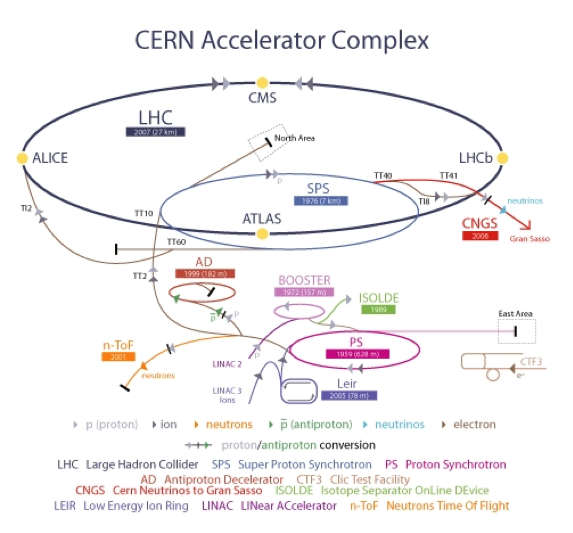
\includegraphics[width=0.85\textwidth]{plots/lhc.png}
\caption{Schematic of the CERN accelerator complex including intermediate accelerators that deliver the proton beams used in the LHC.}
\label{fig:lhc}
\end{center}
\end{figure*}

The proton is a composite particle, which in addition to having three ``valence'' quarks contains more sub-structure in the form of virtual quarks and gluons. 
In Section \ref{sec:qcd} it was shown that gluons interact with both themselves and quarks, thus the gluons that hold the proton together are responsible for producing quark-antiquark pairs which exist inside the proton.
The individual components, or partons, of the proton will each carry some fraction of the total momentum of the proton which is given by the parton distribution function (pdf) and is dependent on the energy of the proton.
In a hadron collision it is in fact the partons that produce the interaction rather that the proton itself.
The pdfs give the probability of finding a particular parton with longitudinal momentum fraction $x$ at a given momentum $Q$. 
Two example pdfs are shown in Figure \ref{fig:pdf}, one for low $Q$ and one for high $Q$.
Upon examination of Figure \ref{fig:pdf} one can see that as the energy of the proton increases, so too does the fraction of the momentum carried by the gluons.
At the energy of the LHC the pdf of the proton is dominated by gluons. 
%In comparison to the LHC, at the energy of the Tevatron the quarks carry a larger fraction of the momentum.
%For this reason colliding protons at the LHC would be somewhat equivalent to colliding protons and antiprotons, as it is more often that the interactions observed are provided by interacting gluons.
At the energy of the LHC, the dominance of the gluon in the pdf means that the majority of interactions are due to two gluons. 
Thus, there is little advantage in colliding protons and anti-protons.
This combined with the fact that antiprotons are difficult to produce and store leads to the conclusion that a proton-proton collider at the LHC energy scale is the logical choice.
\begin{figure*}[htpb]
\begin{center}
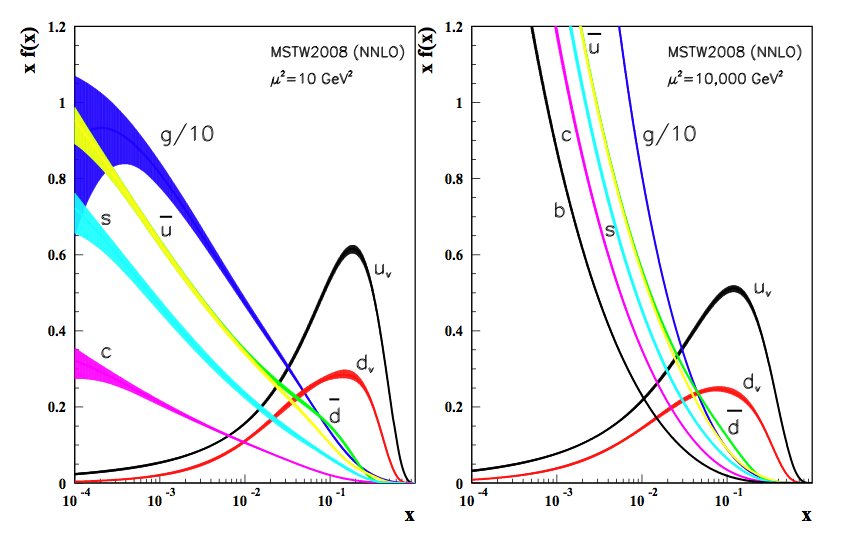
\includegraphics[width=0.85\textwidth]{plots/pdf.png}
\caption{Distributions of $x$ times the parton fraction $f(x)$ for the constituents of the proton at $Q^{2} = 10$ GeV$^{2}$ (left) and $Q^{2} = 10,000$ GeV$^{2}$\cite{PDGREVIEW}.}
\label{fig:pdf}
\end{center}
\end{figure*}


The collision of two protons rather than protons and antiprotons, while negating the difficulty of producing and storing antiprotons, leads to other difficulties.
The colliding particles now have the same charge and as such cannot share the same steering magnets. 
Two separate beam pipes and magnet systems must be used to steer the protons around the LHC ring in different directions.
An additional difficulty at the LHC is the energy at which the protons must be collided in order to probe new physics.
In order to steer the proton beams at an energy of $7$ TeV, dipole magnets are used which must be capable of providing greater than $8$ T magnetic fields.
The superconducting dipole magnets are made of \ce{NbTi} cables that are cooled to superfluid temperatures of $\sim2$ K.
An important aspect of superconducting magnets is quenching, or the process by which the magnet returns to a normal resistive state.
Quenching can occur due to heat dissipation inside the magnet.
A quench can be induced by increasing the current of the magnet, and as a result heat dissipation in the magnet will raise the temperature beyond the critical temperature of the material.
Upon re-energizing the magnet, a greater field can be achieved before a quench occurs, this process is referred to as a training quench.
Due to the number of training quenches required to bend the proton beams at their full $7$ TeV energy, it was decided to operate the accelerator with proton beams of $3.5$ TeV during the 2010 and 2011 data collection periods.
The data collection period of 2012 will see the beam energy increase to $8$ TeV, with the beam increasing to the design energy some time after the maintenance period of 2013-2014.

The magnitude of the Higgs signal to that of common QCD multi-jet events was shown in Section \ref{sec:history}, and similar situations exist for other new physics signals.
%The relative production rates of new physics and the QCD multi-jet processes is what drives the desire to operate the LHC at very high instantaneous luminosities.
In order to probe these rare processes a large number of interactions must be produced in order to collect statistically significant samples, thus the drive for very high integrated luminosities is demonstrated.
During the 2010 data collection period a total integrated luminosity of $36$ pb$^{-1}$ was collected, while during the 2011 data collection period a total integrated luminosity of $4.6$ fb$^{-1}$ was collected.
The integrated luminosity of the 2012 data collection period is projected to be in the range of $15$-$20$ fb$^{-1}$.
The schedule for the increase in luminosity at the LHC is enumerated in Table \ref{tab:lhcluminosity}.
In order to achieve a high luminosity, protons are grouped into high density ``bunches'' made up of multiple protons that are accelerated around the LHC ring. 
By bunching the protons together the probability of two protons having a hard scatter, or collision, is increased.
The luminosity can then be increased by increasing the number of protons in each bunch, thus increasing the number of interacting protons per collision, $N_{1}$ and $N_{2}$ for either beam.
The luminosity can further be increased by placing a larger number of bunches ($n$) in the LHC ring leading to a higher collision rate.
Finally the cross sectional area ($A$) of the beam is minimized at the collision points to maximize the probability of a collision. 
These three factors can be seen in the following equation that gives the instantaneous luminosity,
\begin{equation}
\Lagr = fn\frac{N_{1}N_{2}}{A}.
\end{equation}
A side effect of increasing the luminosity in this way is that while increasing the probability of an interesting collision, the probability of ``uninteresting'' collisions is also increased.
In fact it is common for multiple interactions to occur in the same bunch, up to $\sim 35$ in some cases for the 2011 data collection.
This presents a challenge to an analysis performed at a hadron collider in that each event contains an effective ``pile-up'' of multiple events that must be taken into account when searching for new physics.

\begin{table}[htpb]
\begin{center}
\caption{LHC LUMINOSITY INCREASE SCHEDULE}
\begin{tabular}{lc}
\toprule
Year & Integrated Luminosity [fb$^{-1}$] \\
\midrule
2010 & $0.036$ \\
2011 & $4.6$ \\
2012 & $15$-$20$(projected) \\
\bottomrule
\end{tabular}
\label{tab:lhcluminosity}
\end{center}
\end{table}
% magnets
% proton-proton
% luminosity


\section{Superconducting Magnet}
\label{sec:magnet}
As the name the Compact Muon Solenoid implies the superconducting solenoid magnet is a central feature of the CMS detector.
The magnetic field is necessary to measure the momentum of charged particles produced in the proton-proton collisions.
As a charged particle travels through a magnetic field the radius of curvature for the charged particle is given by
\begin{equation}
r = {p_{\perp}\over|q|B},
\end{equation}
where $p_{\perp}$ is the component of the particle's momentum that is transverse to the direction of the magnetic field, $q$ is the charge of the particle, and B is the strength of the magnetic field.
As the radius of curvature is proportional to $p_{\perp}$, it becomes clear that to measure high momentum particles a very large magnetic field is required.
In addition to the requirement for the magnetic field to be large, it is also important that magnetic field be homogeneous in the volume of the detector to reduce systematic errors that result from a non-uniform field.

In order to provide a homogeneous magnetic field the CMS solenoid is required to be physically large, encapsulating the tracking system and calorimeters.
It has a radial bore of 6.3 meters, a length of 12.9 meters, and a weight of 220 tons.
The solenoid is made of four layers of wire with a total of 2168 turns carrying a nominal current of 19.14 kA.
A second momentum measurement is applied to muons that are detected in the muon system surrounding the solenoid, for this reason the muon system is interspersed throughout the iron return yoke.
The return yoke has the effect of minimizing the fringe field outside the solenoid, providing a homogeneous field throughout the muon system. %FIXME return yoke necessary

\section{Charged Particle Tracking System}
\label{sec:tracker}
The charged particle tracking system is the sub-detector that lies closest to the beam pipe.
Its purpose is to measure the the trajectories of charged particles that emerge from the collisions.
The trajectories are then used to determine the momentum and charge of the charged particles.
In order to measure the trajectories several layers of silicon detectors are used, as charged particles traverse these layers they create electronic signals in the silicon.
Each of these signals, often referred to as ``hits'', correspond to the position of a charged particle as it travels through the detector.
The hits that are measured in the tracking system are fit to a helix producing the trajectories that are used to measure the charge and momentum.
For high momentum tracks the tracking system provides very good resolution for the transverse momentum of approximately $1-2\%$ in the barrel region, while in the endcap region ($|\eta| > \sim1.5$) the resolution degrades as can be seen in Figure \ref{fig:trackerptres}.
\begin{figure}[htpb]
\begin{center}
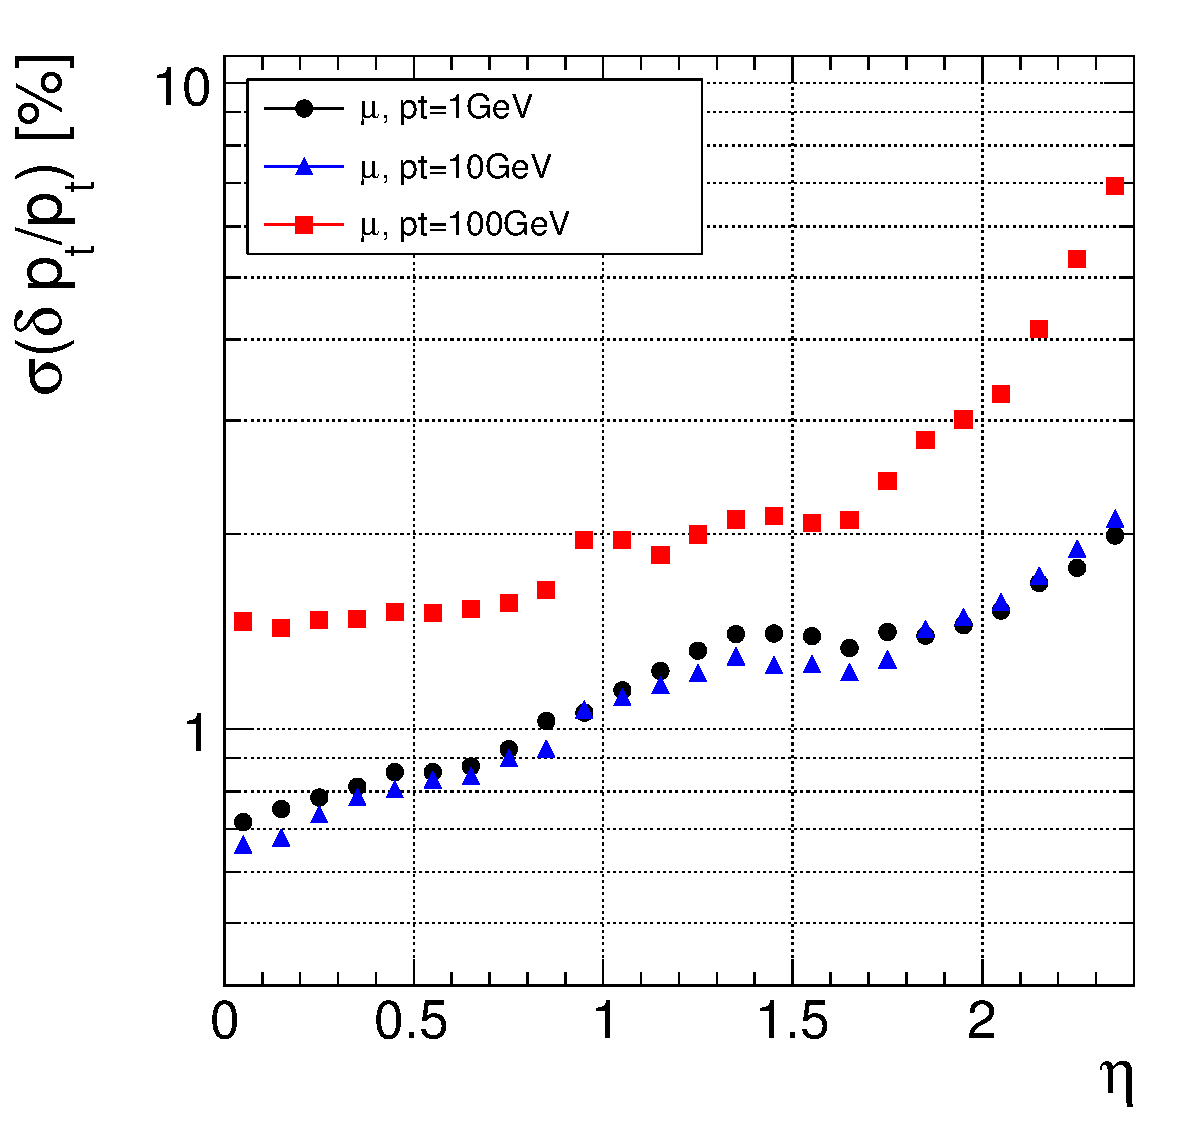
\includegraphics[width=0.85\textwidth]{plots/trackerptres.pdf}
\caption{Transverse momentum resolution of the CMS tracking system as a function of pseudo-rapidity ($\eta$) for muons with $p_{T} = 1$, $10$, and $100$ GeV\cite{CMS_DETECTOR}.}
\label{fig:trackerptres}
\end{center}
\end{figure}

The tracking system is designed to have the capacity of measuring secondary decay vertices, for example, arising from the decay of bottom quarks and tau leptons.
Bottom quarks and tau leptons have relatively long life times, as such they travel a non-negligible distance before decaying, giving rise to secondary decay vertices.
In order to measure secondary decay vertices, the tracking system is constructed using two technologies, an inner tracking system consisting of silicon pixel detectors and an outer tracking system of silicon strips.
The inner layer of the pixel tracking system is placed at a radius of $4.4$ cm in order to be as close as possible to the interaction point.
This pixel tracking system is made up of three layers in the barrel and two layers in the endcaps.
Outside the pixel tracking system is the silicon strip tracking system consisting of ten layers of silicon strips in the barrel region and 12 layers in the endcaps. 
A schematic of the CMS tracking system can be seen in Figure \ref{fig:trackerlayout}.
The transverse impact parameter ($d_{0}$) resolution of the tracking system gives an indication of the performance one can expect for the secondary decay vertex reconstruction, for high momentum tracks the resolution is approximately $10$ \micrometer as can be seen in Figure \ref{fig:trackerd0res}. %FIXME micrometer
For lower momentum tracks the resolution of $d_{0}$ degrades due to multiple scattering of the particle in the tracker material.
\begin{figure}[htpb]
\begin{center}
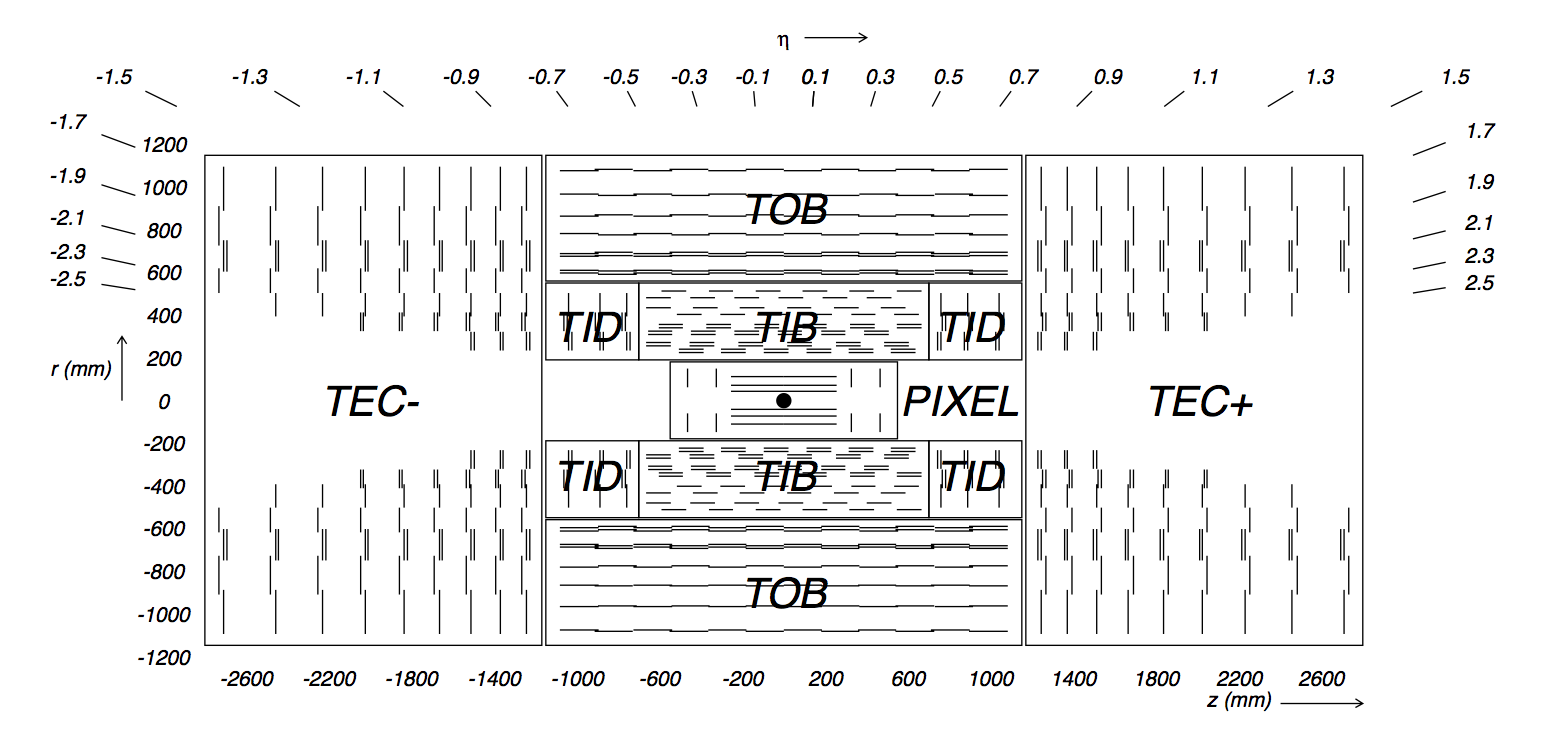
\includegraphics[width=0.85\textwidth]{plots/trackerlayout.png}
\caption{Schematic of the CMS inner tracking system\cite{CMS_DETECTOR}. The barrel tracker is divided into the Tracker Inner Barrel (TIB) and Tracker Outer Barrel (TOB). The endcap tracker is divided into the Tracker End Cap (TEC) and Tracker Inner Disks (TID).}
\label{fig:trackerlayout}
\end{center}
\end{figure}

\begin{figure}[htpb]
\begin{center}
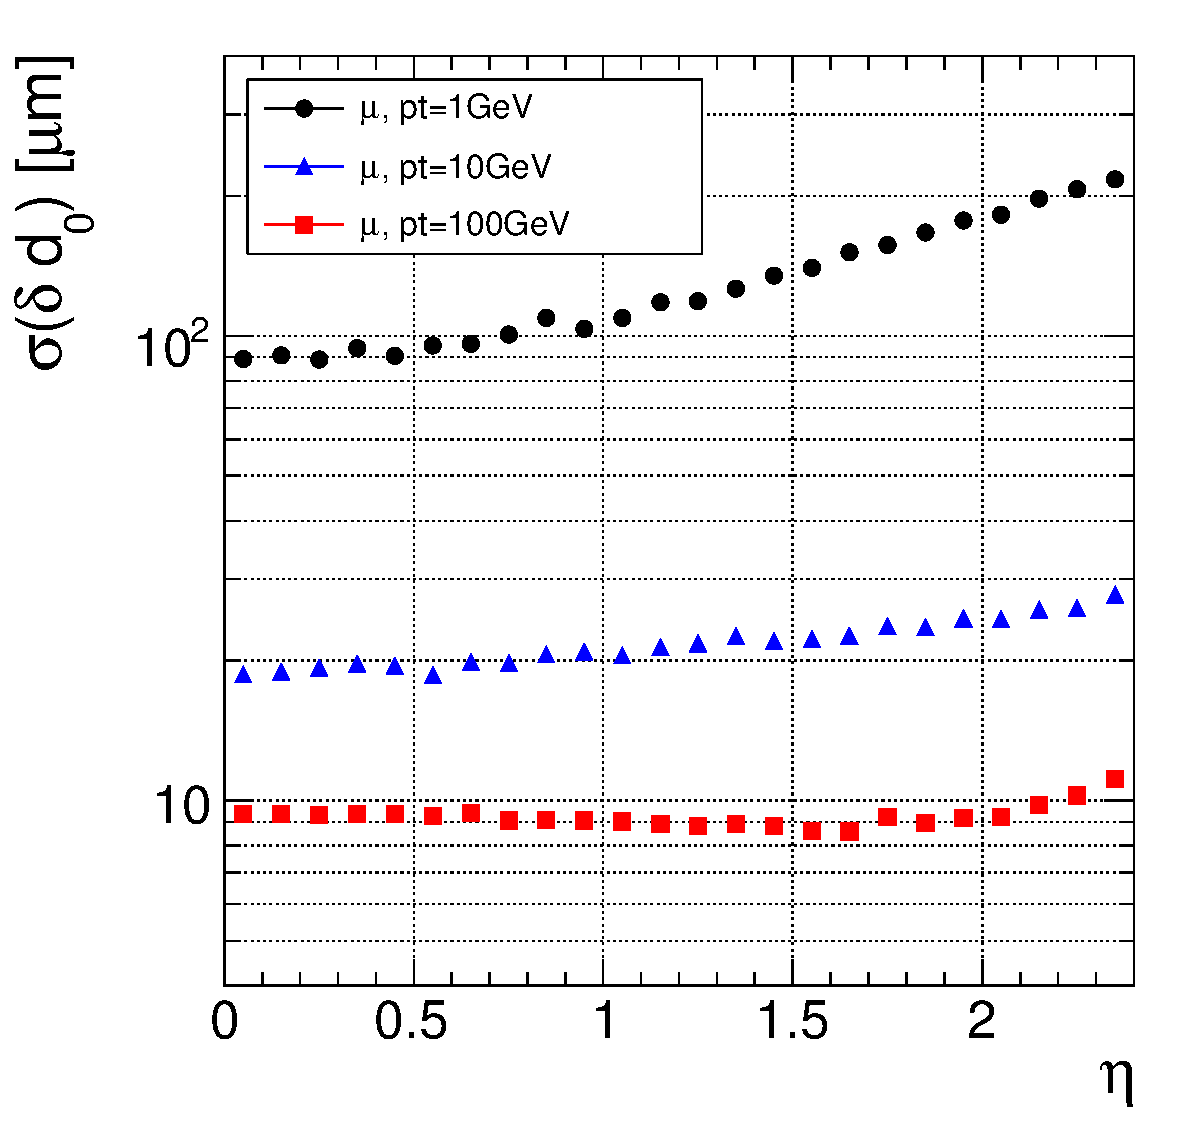
\includegraphics[width=0.85\textwidth]{plots/trackerd0res.pdf}
\caption{Transverse impact parameter resolution of the CMS tracking system a function of pseudo-rapidity ($\eta$) for muons with $p_{T} = 1$, $10$, and $100$ GeV\cite{CMS_DETECTOR}.}
\label{fig:trackerd0res}
\end{center}
\end{figure}

Both the inner and outer tracking systems consist entirely of silicon, which operate by doping the silicon and thus creating a diode. % FIXME reword?
A reverse bias is then applied to the silicon to deplete the region, so that when a charged particle passes through the silicon a small ionization current is induced which can then be measured.
The most common method of forming this type of silicon diode is to create a p-n junction, however to ensure radiation hardness the layering in the tracking system silicon is more complicated\cite{CMS_DETECTOR}. %FIXME involves creating
In order to achieve high resolution track measurements suitable for the measurement of secondary decay vertices and particle impact parameters, the pixels in the inner layers are electronically isolated and constructed in sizes of $100$x$150$ \micrometer.
The tracking system was designed such that the occupancy would be less than or equal to 1\% at the design luminosity, and as such the outer tracking system does not need to be as finely divided as the inner pixel system.
The outer tracking system is constructed of silicon strips providing single point resolution between $23$ to $52$ \micrometer in both $r$-$\phi$ and $z$ directions.

Tracks are reconstructed from the reconstructed hits in the tracker by means of the Combinatorial Track Finder (CTF) algorithm\cite{TRACKRECO}.
The CTF begins by first locating pairs of reconstructed hits in the inner pixel detector that are compatible with the interaction region.
The track finding then uses a Kalman filtering method to combine the seeded parameters with nearby reconstructed hits.
During each step of the finding algorithm each track is assigned a quality, ambiguities that arise from two tracks are resolved by rejecting the track that is of lesser quality.
Once the track finding method is complete each track undergoes two least squares fitting procedures, the first is an inside-out fit that serves to remove any approximations or biases that arise from the seeding or finding algorithms.
The second fit is an outside-in fit that serves to smooth the final track.
The final track finding procedure is performed iteratively to improve the efficiency of the track finding process, the CTF is repeated three to four times.
After each iteration of the CTF a set of filters is applied setting aside high quality tracks and removing their reconstructed hits from the next iteration.
The iterative procedure has been shown to increase the track finding efficiency by approximately $5\%$ while keeping mis-identification rates low.
Further, the iterative procedure also allows for the reconstruction of low momentum tracks that would otherwise not be reconstructed with a single CTF.

\section{Electromagnetic Calorimeter}
\label{sec:ecal}
The electromagnetic calorimeter (ECAL) was designed with the specification of measuring the energy of particles that interact electromagnetically with a very high precision. 
The search for the Higgs boson in the channel $H\rightarrow\gamma\gamma$ was a driving factor in the design of the ECAL.
The ECAL is a hermetic, homogeneous detector constructed of scintillating lead tungstate (\ce{PbWO4}) crystals, 61200 in the barrel region, and 7324 in each of the endcaps.
Particles that interact electromagnetically, primarily electrons and photons, will cause electromagnetic showers in the ECAL material.
An electromagnetic shower is a process in which electrons and photons are created, via pair-production or bremsstrahlung respectively.
The ultimate conclusion of an electromagnetic shower is a collection of scintillation photons that are measured by photo multipliers which read out the signal of each crystal. %FIXME diodes?
The energy of the particle inducing the shower can be inferred from the number of photons that are collected.

To reliably measure the energy of an incident electron or photon, the total energy of the particle must be absorbed by the calorimeter, and thus a crystal must be capable of capturing the entire shower of a particle longitudinally.
The ability of the crystal to confine an electromagnetic shower is dependent on the depth of the crystal, the density of the crystal, and the radiation length of an electromagnetic shower in the material.
The radiation length ($X_{0}$) is a unit of measurement defined by the mean distance that an electron must travel before its energy is reduced by $(1-{1\over e})$.
These criteria were the driving choice in the decision to use \ce{PbWO4} crystals as this material is very dense, leading to maximal shower capture while maintaining a compact size.
The crystals used have a density of $8.28$ g/cm$^{3}$ and a length of $230$ mm resulting in a total radiation length of $25.8 X_{0}$
The Moliere radius is the lateral distance in which 90\% of an electromagnetic shower is contained. for \ce{PbWO4} this radius is $22$ mm. 
The inner facing cross section of the ecal crystals is $22\times22$ mm, such that if an incident particle were to hit the center of a crystal 90\% of the particle's energy would be contained in a single crystal.

% Transparency? FIXME

Below energies of $500$ GeV the energy resolution of the ECAL can be parameterized as a function of energy,
\begin{equation}
\label{eq:ecalresolution}
\left({\sigma \over E}\right)^{2} = \left({S \over \sqrt{E}}\right)^{2} + \left({N \over E}\right)^{2} + C^{2},
\end{equation}
where $S$ is the stochastic noise term, $N$ is the noise term, and $C$ is a constant.
The resolution of the ECAL as a function of energy was determined in 2004 by fitting the measured energy to Equation \ref{eq:ecalresolution} in a test beam of electrons with energies ranging from $20$ GeV to $250$ GeV, the results of the fit can be seen in Figure \ref{fig:ecalres}.
For energies above $20$ GeV the energy resolution of the ECAL is better than $1\%$\cite{CMS_DETECTOR}.
\begin{figure}[htpb]
\begin{center}
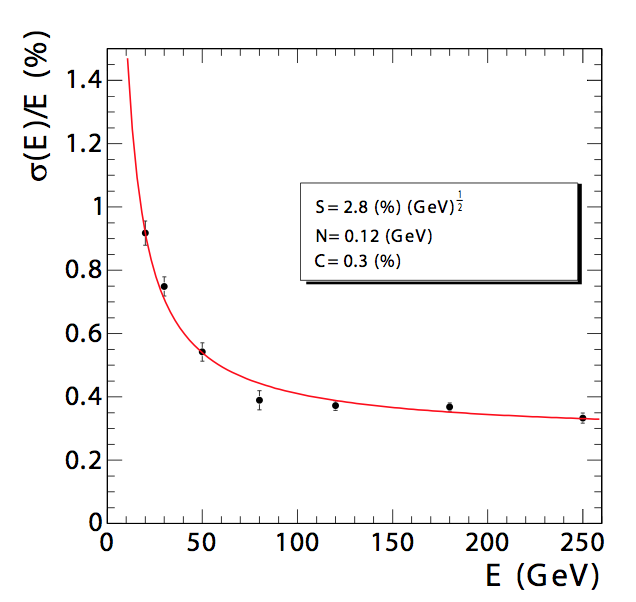
\includegraphics[width=0.85\textwidth]{plots/ecalres.png}
\caption{The CMS detector electromagnetic calorimeter energy resolution as a function of electron energy\cite{CMS_DETECTOR}.}
\label{fig:ecalres}
\end{center}
\end{figure}

\section{Hadronic Calorimeter}
\label{sec:hcal}
The hadronic calorimeter (HCAL) is designed to measure the energy of hadrons while providing good shower containment and hermicity.
The HCAL surrounds the ECAL and is inside the solenoid, with the exception of the hadronic outer (HO) detector which is placed just outside the solenoid.
The purpose of the HO is to catch any hadronic showers which are not fully contained within the bulk of the HCAL.
A schematic of the HCAL subsystem layout is shown in Figure \ref{fig:hcallayout}.
The HCAL is a sampling calorimeter in that it utilizes scintillating plastic tiles with embedded wavelength-shifting fibers (WLS), interspersed between brass absorber plates.
A hadron traveling through the HCAL will interact with the brass absorber producing a hadronic shower which produces photons as the particles in the shower pass through the scintillating tiles.
The photons captured in the tiles are then carried via the WLS to the hybrid photodiode based readout system.
%As the HCAL is a sampling calorimeter the radial profile of the hadronic shower can be measured by using each of the tiles separately giving an additional parameter to the measurement of the deposited energy.
\begin{figure}[htpb]
\begin{center}
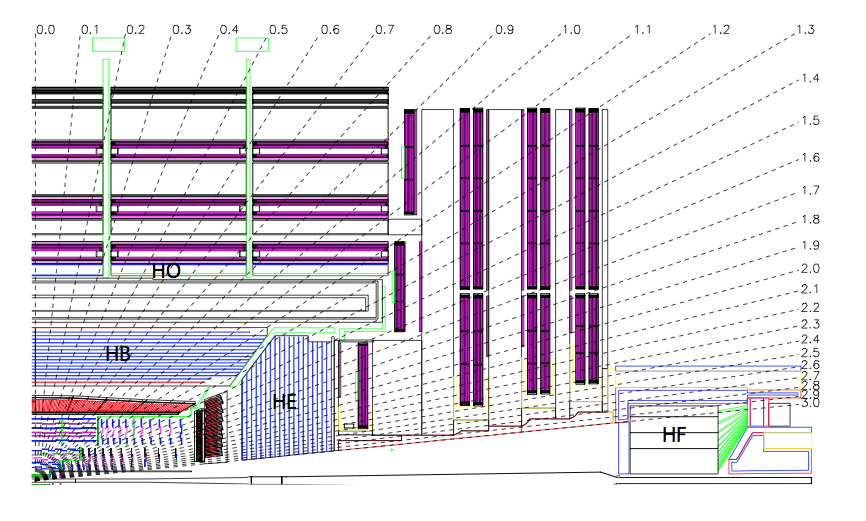
\includegraphics[width=0.9\textwidth]{plots/hcallayout.png}
\caption{Schematic of the CMS hadronic calorimeter subsystem\cite{CMS_DETECTOR}.}
\label{fig:hcallayout}
\end{center}
\end{figure}

A forward calorimeter (HF) is used in addition to the HCAL barrel, endcaps, and HO. 
The HF spans the region from $\pm3.0$ to $\pm5.0$ in $\eta$, and is designed to measure the hadronic energy deposited in the congested high $\eta$ region.
Not only does the HF provide the ability to measure hadronic energy in the high $\eta$ regions, but also provides a method to measure the luminosity delivered to the CMS detector.
The HF is a Cherenkov detector with quartz fibers, running parallel to the beam line,  installed into grooves situated inside a steel absorber.
Hadronic showers that originate in the steel absorber will contain neutral and charged particles that will produce Cherenkov light if their energy is above a certain threshold.
The Cherenkov light is then measured to reconstruct the energy deposited in the calorimeter.
The quartz fibers used have two lengths where one length is shorter than the other, providing a means of separating electrons and photons from hadrons.
This is possible as showers produced from incident electrons and photons will deposit their energy very quickly and not travel as far as showers produced from incident hadrons.

The jet $E_{T}$ resolution as a function of transverse energy is shown in Figure \ref{fig:jetres}. The $E_{T}$ resolution is better than $20\%$ for jets with $E_{T} > 50$ GeV, and drops to $10\%$ for jets with $E_{T} > 300$ GeV.
\begin{figure}[htpb]
\begin{center}
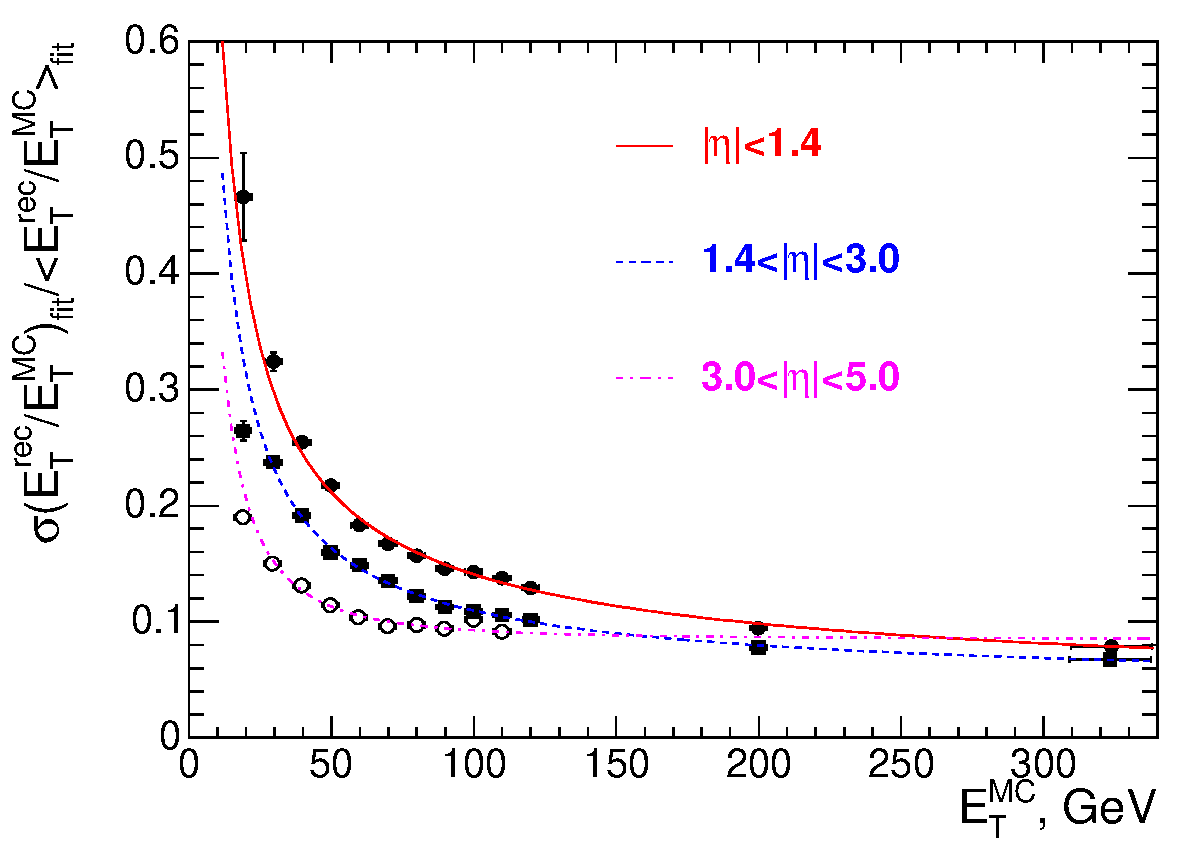
\includegraphics[width=0.85\textwidth]{plots/jetres.pdf}
\caption{Jet energy resolution for the HCAL in the barrel, endcap and forward regions\cite{CMS_DETECTOR}.}
\label{fig:jetres}
\end{center}
\end{figure}

\section{Muon System}
\label{sec:muonsystem}
The detection of muons is a powerful tool at hadron colliders because they leave a unique signal in the detector.
The signal is unique for a couple of reasons:
\begin{itemize}
\item A muon is charged so a muon's momentum can be measured via its trajectory.
\item A muon is a minimum ionizing particle so it will be one of the few particles that does not leave much energy in the calorimeter systems.
\end{itemize}
The muon system for the CMS detector is situated in the iron return yoke of the solenoid. 
Although the components of the muon system are different than that of the tracking system, it reconstructs charged particle tracks in a similar manner.
Being situated outside of the calorimeters and solenoid, all other particles that would otherwise interact with the muon system are stopped before reaching it.
A muon can be identified by matching a track in the inner tracking system to a track in the muon system.
Further, a muon can be more cleanly identified by restricting the amount of energy deposited near the muon in either of the calorimeters.

In the barrel region ($|\eta| < 1.2$) the muon system is primarily composed of Drift Tube (DT) chambers.
A drift tube is constructed by running a wire carrying a positive current through a tube filled with an inert gas.
When a charged particle enters the tube it will ionize the gas and the free electrons will be attracted to the wire, generating a signal that can be measured.
In the case of the CMS detector DTs, the gas is a mixture of 85\% Argon/15\% Carbon Dioxide, and the wires are held at a voltage of $3.6$ kV.
The muon barrel DT system is separated into five wheels each with four concentric layers where the inner three layers measure track positions in $r$, $\phi$ and $z$, while the outer most layer does not measure the $z$ coordinate.
The three inner cylinders are comprised of 60 drift chambers while the outer cylinder consists of 70 drift chambers for a total of approximately $172,000$ sensitive wires. 
A schematic of a muon DT wheel is shown in Figure \ref{fig:dtlayout}.
\begin{figure}[htpb]
\begin{center}
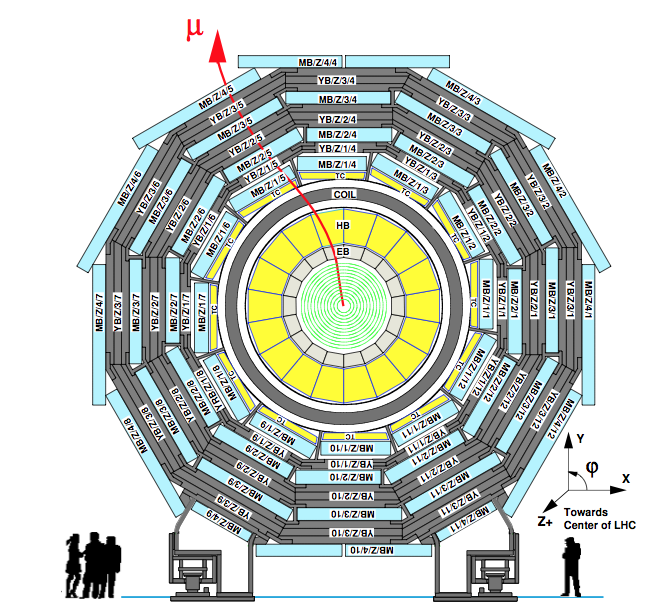
\includegraphics[width=0.9\textwidth]{plots/dtlayout.png}
\caption{Schematic of the CMS barrel muon DT chambers\cite{CMS_DETECTOR}.}
\label{fig:dtlayout}
\end{center}
\end{figure}

Cathode strip chambers (CSC) are used in the endcap regions, extending the coverage to $|\eta| < 2.4$. 
The CSC detectors are trapezoidal chambers filled with an inert gas.
Each chamber contains a plane of cathode strips organized radially, and a plane of anode wires held at high voltage running nearly perpendicular to the strips.
When a muon passes through one of the cathode strip chambers it will ionize the gas.
Once the gas has been ionized, an avalanche current will be created between an anode wire and a number of the cathode strips which can then be measured.
Using the measurement of the signal on the anode wire provides a signal that is fast enough to be used as a trigger sample, however, yields the relatively poor $r-\phi$ spatial resolution of $2$ mm.
The offline reconstructed position of the muon can be measured much more precisely by taking the average of the charge distribution on the cathode strips and the position of the anode wire.
Using the cathode strips as well as the anode wires provides a spatial resolution of $75$ \micrometer in the first layer and $150$ \micrometer in the outer layers.
The CSCs are distributed in the endcap region such that each chamber covers either $10^{\circ}$ or $20^{\circ}$ in $\phi$ and overlap to eliminate any gaps in $\phi$ coverage for the system.
The layout for the CSCs can be seen in Figure \ref{fig:csclayout}.
\begin{figure}[htpb]
\begin{center}
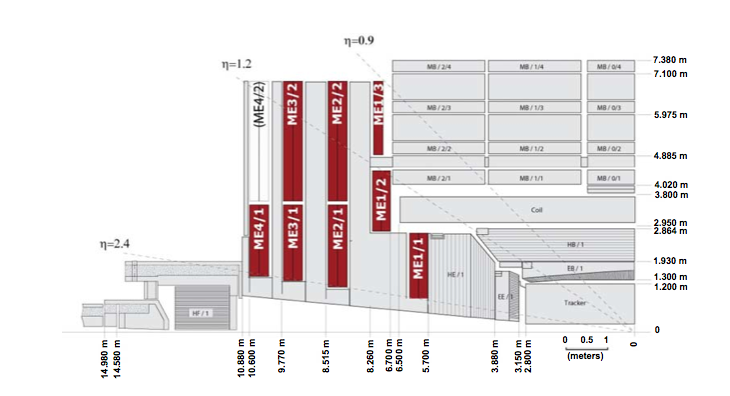
\includegraphics[width=0.9\textwidth]{plots/csclayout.png}
\caption{Schematic of the CMS muon system with the CSC chambers highlighted in red\cite{CMS_DETECTOR}.}
\label{fig:csclayout}
\end{center}
\end{figure}


As both the DT and CSC muon sub systems are relatively slow compared to the speed needed for the trigger system to correctly identify the associated bunch crossing with a triggered muon, an additional sub system exists to provide the muon system with the capability of providing a fast first level trigger.
The Resistive Plate Chamber (RPC) is a gaseous parallel-plate detector that provides a time resolution comparable to that of a scintillator\cite{RPC}.
The muon RPCs extend to $|\eta| \le 1.6$ covering the muon system barrel region and a portion of the endcap region. 
The layout of the RPCs is shown in Figure \ref{fig:rpclayout}.
The RPCs are capable of providing an estimate of the transverse momentum for a muon on a very short time scale that can unambiguously be matched to a bunch crossing even in the presence of the high rates and pile-up seen at the LHC.
Each chamber consists of two gaps (up/down) of $2$ mm operated in avalanche mode with a common read out strip between them, this provides a higher efficiency than would be obtainable with a single gap while allowing for a lower operating voltage. % FIXME MORE EXPLANATION
The RPC chambers utilize a gas mixture of $96.2\%$ \ce{C2H2F4}, $3.5\%$ \ce{iC4H10}, and $0.3\%$ \ce{SF6}.
% FIXME radiation?
\begin{figure}[htpb]
\begin{center}
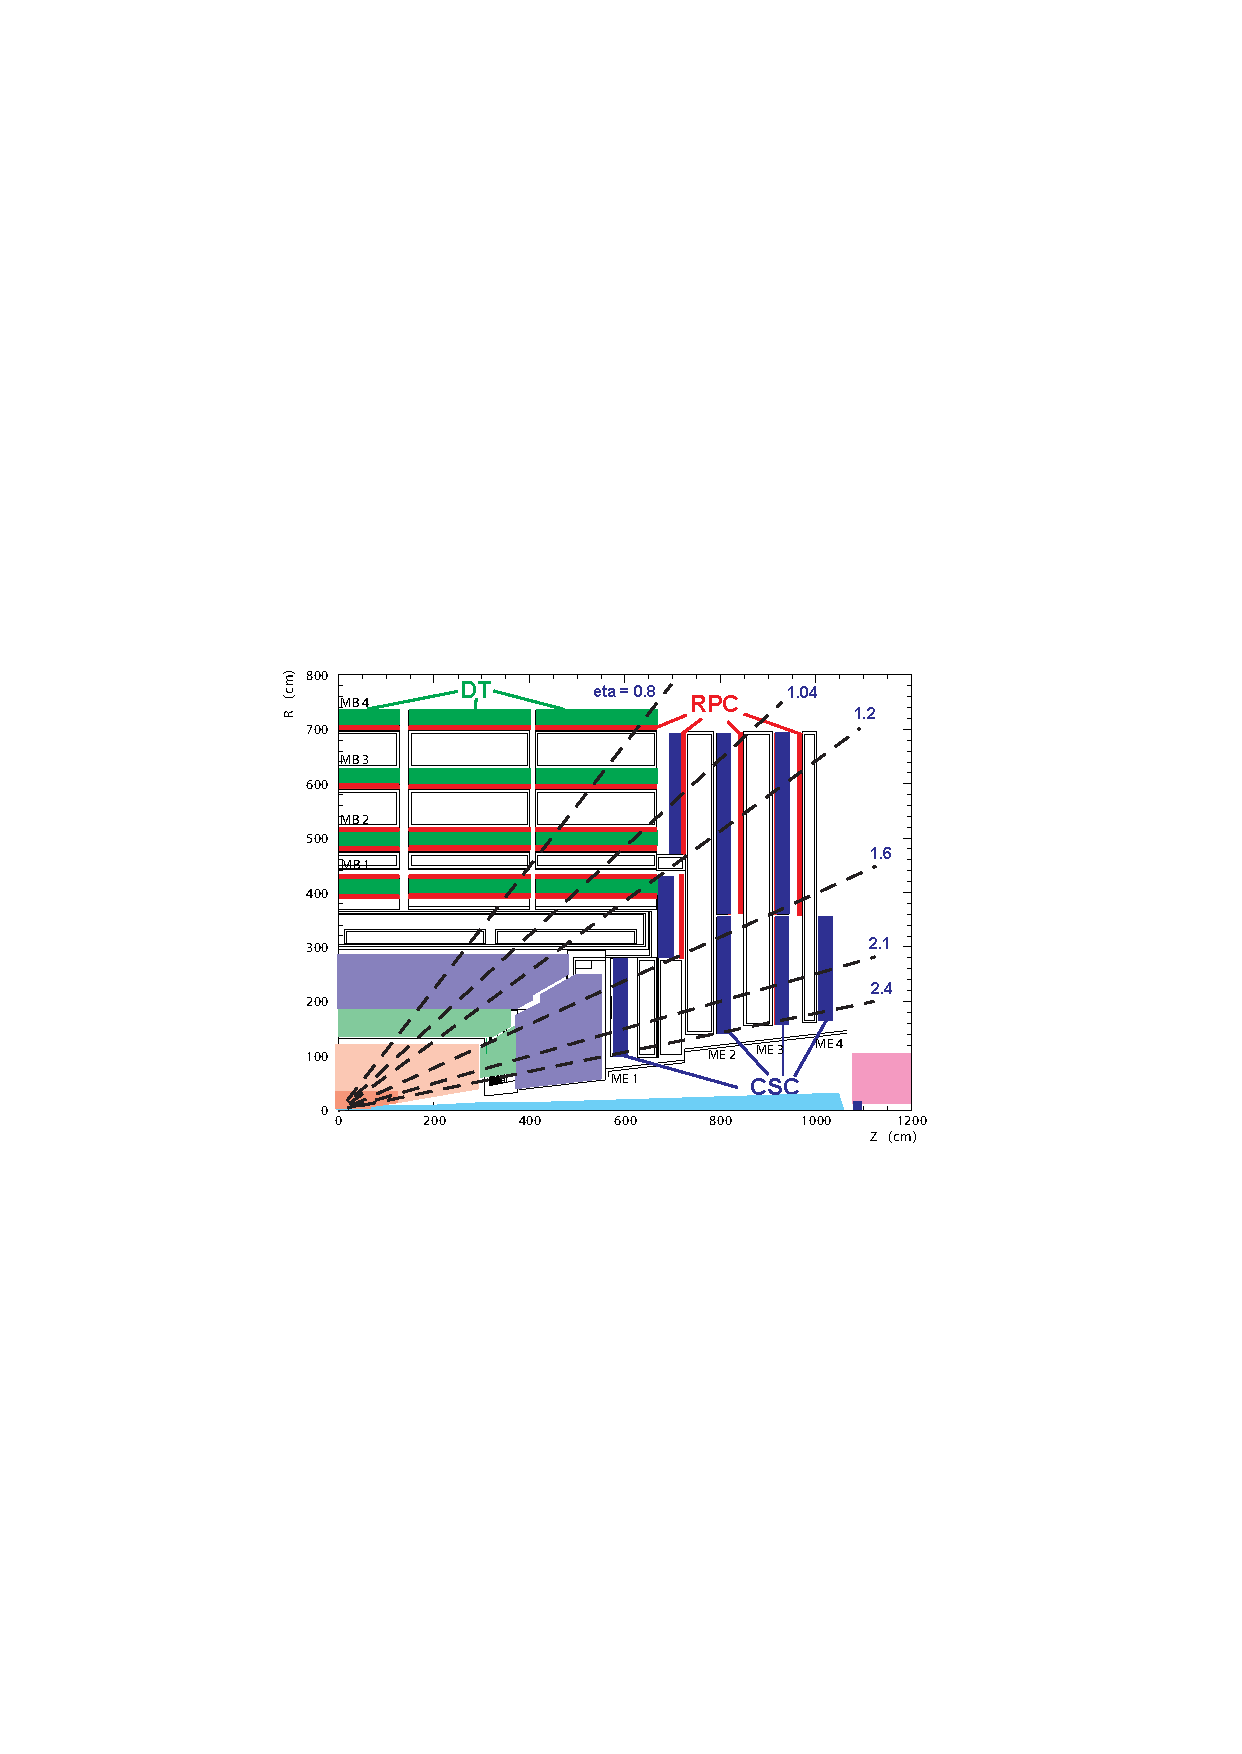
\includegraphics[width=0.9\textwidth]{plots/rpclayout.pdf}
\caption{Schematic of the CMS muon system\cite{TDR}.}
\label{fig:rpclayout}
\end{center}
\end{figure}

The resolution of muon momentum measurements suffers from multiple scattering in the detector material before the muon system.
The momentum resolution of the muon system is in the range of approximately $9\%$-$45\%$ depending on the $p$ and $\eta$.
This situation can be vastly improved, however, by performing a global momentum fit to the track measured in the inner tracker with the track measured in the muon system.
Figure \ref{fig:muonres} shows that the momentum resolution is improved by an order of magnitude for low $p_{T}$ and $\eta$ with a substantial improvement for high $p_{T}$ and $\eta$. 
In addition to performing a global fit, two independent measurements of the muon $p_{T}$ can provide a useful cross-check on the measured momentum.
\begin{figure}[htpb]
\begin{center}
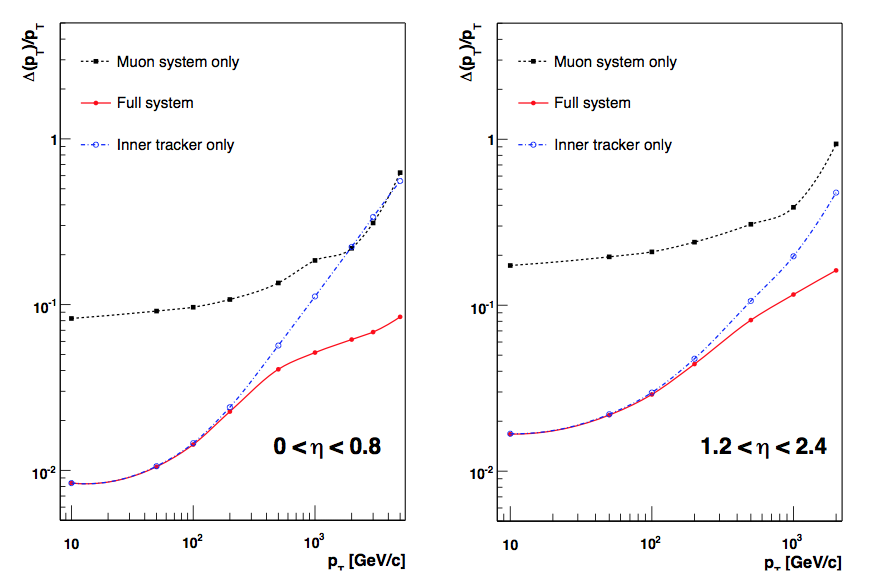
\includegraphics[width=0.9\textwidth]{plots/muonres.png}
\caption{Comparison of muon momentum resolution using the inner tracking system alone, the muon system alone, and the inner tracking system combined with the muon system for the barrel (left) and endcap (right) regions\cite{CMS_DETECTOR}.}
\label{fig:muonres}
\end{center}
\end{figure}

% RPC

\section{Trigger System}
\label{sec:triggersystem}
%At the nominal LHC luminosity of $10^{34}$ \lumiunit, bunch crossings will occur every 25 ns, which would correspond to an interaction rate of approximately $40$ MHz.
At the LHC design specifications, bunch crossings will occur every 25 ns. 
This rate would correspond to an interaction rate of approximately $40$ MHz.
Considering the complexity of the CMS detector, the bandwidth required to read and store data from every bunch crossing would be greater that one Petabit per second.
In addition to the unrealistic requirements of storing every event, is the fact that the cross section for common QCD interactions is many orders of magnitude larger than that of ``interesting'' physics.
These reasons lead to the obvious solution that there must be a system by which interesting events are kept, and common events are discarded.
The CMS trigger system is designed with this task in mind and consists of a very fast first-level trigger (L1), and a  more complete high level trigger (HLT).

The designed acceptance rate of the L1 trigger is $100$ kHz. 
In order to achieve this the L1 trigger is comprised of custom electronics that are built into the subdetector subsystems.
The latency of the L1 trigger is restricted to $3.2$ \microunit{s} and as such only information from the calorimeters and muon system are available, as the time constraint on reconstructing tracks is too great.
Each subdetector system generates a set of trigger primitives, typically photon/electron objects, muons and jets with certain $E_{T}$ or $p_{T}$ thresholds.
The L1 trigger also integrates global requirements such as sums over transverse energy ($E_{T}$) and missing transverse energy ($\met$) from the calorimeters.
After a successful L1 trigger decision, the event is fed into memory pipelines for read out by the Data Acquisition System (DAQ) and ultimately the HLT.
Unlike the L1 trigger which relies on fast dedicated hardware, the HLT is run in software on a farm of commercial computers.
The acceptance rate of the HLT is required to be on the order of $100$ Hz giving room for more complex operations such as reconstructing tracks, but the time to analyze each collision remains tight.
The HLT is made up of several ``paths'' that typically represent more complex versions/combinations of the L1 trigger primitives, such as a single photon with a given $E_{T}$ threshold or a muon and tau in coincidence.
Running the HLT in software allows for a greater flexibility to meet changing demands based on requirements such as increasing luminosity, or even hints towards new physics.

This analysis uses a cross trigger which requires both a muon and a hadronically decaying tau to be present in order to pass the HLT.
The triggers used are all based upon a single muon L1 seed, then in the HLT path both a muon and a tau object are required to be present.
In order to reduce rates as the luminosity increased over the 2011 running period, several different triggers were used throughout different run ranges. 
The triggers used will be described in more detail in Chapter \ref{chap:analysis}.


\section{Simulation}
\label{sec:simulation}
Several Monte Carlo simulations are used to compare the data to theoretical expectations for both the signal and background processes.
The simulated events are produced via the PYTHIA\cite{PYTHIA} or MADGRAPH\cite{MADGRAPH} event generators.
These are software tools that generate simulations of the hard scattering parton events as seen at the LHC and the Tevatron. 
They both use leading-order (LO) matrix elements.
By interfacing POWHEG\cite{POWHEG} with PYTHIA one can combine the parton shower generator with next-to-leading-order (NLO) QCD computations, providing an accurate description of the event while taking into account initial and final state radiation.
For samples which require the simulation of a tau lepton decay, the software package Tauola\cite{TAUOLA} is used.
The Tauola software package uses the matrix elements specifically associated with tau lepton decays to provide an accurate simulation of the processes involved.
A summary of the datasets used can be found in Tables \ref{tab:backgroundsimulations} and \ref{tab:signalsimulations} for background and signal processes respectively. 
Once the event has been generated it is run through a detailed GEANT4 based simulation of the detector that produces simulated particle trajectories\cite{GEANT4}.
In addition to particle trajectories, the detector simulation produces a set of simulated digitized signals that are then processed with the same reconstruction algorithms as are run on the data.

\begin{table}[tpb]
  \begin{center}
    \caption{BACKGROUND SIMULATION DATASETS}
    \label{tab:backgroundsimulations}
    \begin{tabular}{lcc}
      \toprule
      Process & Event Generator & Integrated Luminosity [fb$^-1$]\\
      \midrule
      $Z / \gamma^{*} \rightarrow \tau\tau$ & POWHEG + PYTHIA & 12.2\\
      $Z / \gamma^{*} \rightarrow \mu\mu$ & POWHEG + PYTHIA & 18.12\\
      QCD multi-jet & PYTHIA & 0.2\\
      $W+$ multi-jet $\rightarrow l\nu$ & MADGRAPH & 2.6\\
      $WW$ & PYTHIA & 152\\
      $WZ$ & PYTHIA & 406\\
      $t\overline{t} +$ multi-jet & MADGRAPH & 22\\
      \bottomrule
    \end{tabular}
  \end{center}
\end{table}

\begin{table}[tpb]
  \begin{center}
    \caption{SIGNAL SIMULATION DATASETS}
    \label{tab:signalsimulations}
    \begin{tabular}{lc}
      \toprule
      Process & Event Generator \\
      \midrule
      $gg \rightarrow H$ & POWHEG + PYTHIA \\
      $qq \rightarrow Hqq$ & POWHEG + PYTHIA \\
      $gg \rightarrow A$ & PYTHIA \\
      $gg \rightarrow Abb$ & PYTHIA \\
      \bottomrule
    \end{tabular}
  \end{center}
\end{table}


